% ========================================
%	Header einbinden
% ========================================

\documentclass[bibtotoc,titlepage]{scrartcl}

% Deutsche Spracheinstellungen
\usepackage[ngerman,german]{babel, varioref}
\usepackage[T1]{fontenc}
\usepackage[utf8]{inputenc}

%\usepackage{marvosym}

\usepackage{amsfonts}
\usepackage{amssymb}
\usepackage{amsmath}
\usepackage{amscd}
\usepackage{amstext}
\usepackage{float}
\usepackage{caption}
\usepackage{wrapfig}
\usepackage{setspace}
\usepackage{threeparttable}
\usepackage{footnote}

\usepackage{caption}
\usepackage{subcaption}

\newfloat{formel}{htbp}{for}
\floatname{formel}{Formel}


\usepackage{longtable}

%\usepackage{bibgerm}

\usepackage{footnpag}

\usepackage{ifthen}                 %%% package for conditionals in TeX
\usepackage{siunitx}
%Fr textumflossene Bilder und Tablellen
%\usepackage{floatflt} - veraltet

%Fr Testzwecke aktivieren, zeigt labels und refs im Text an.
%\usepackage{showkeys}

% Abstand zwischen zwei Abs�zen nach DIN (1,5 Zeilen)
% \setlength{\parskip}{1.5ex plus0.5ex minus0.5ex}

% Einrckung am Anfang eines neuen Absatzes nach DIN (keine)
%\setlength{\parindent}{0pt}

% R�der definieren
% \setlength{\oddsidemargin}{0.3cm}
% \setlength{\textwidth}{15.6cm}

% bessere Bildunterschriften
%\usepackage[center]{caption2}


% Probleml�ungen beim Umgang mit Gleitumgebungen
\usepackage{float}

% Nummeriert bis zur Strukturstufe 3 (also <section>, <subsection> und <subsubsection>)
%\setcounter{secnumdepth}{3}

% Fhrt das Inhaltsverzeichnis bis zur Strukturstufe 3
%\setcounter{tocdepth}{3}

\usepackage{exscale}

\newenvironment{dsm} {\begin{displaymath}} {\end{displaymath}}
\newenvironment{vars} {\begin{center}\scriptsize} {\normalsize \end{center}}


\newcommand {\en} {\varepsilon_0}               % Epsilon-Null aus der Elektrodynamik
\newcommand {\lap} {\; \mathbf{\Delta}}         % Laplace-Operator
\newcommand {\R} { \mathbb{R} }                 % Menge der reellen Zahlen
\newcommand {\e} { \ \mathbf{e} }               % Eulersche Zahl
\renewcommand {\i} { \mathbf{i} }               % komplexe Zahl i
\newcommand {\N} { \mathbb{N} }                 % Menge der nat. Zahlen
\newcommand {\C} { \mathbb{C} }                 % Menge der kompl. Zahlen
\newcommand {\Z} { \mathbb{Z} }                 % Menge der kompl. Zahlen
\newcommand {\limi}[1]{\lim_{#1 \rightarrow \infty}} % Limes unendlich
\newcommand {\sumi}[1]{\sum_{#1=0}^\infty}
\newcommand {\rot} {\; \mathrm{rot} \,}         % Rotation
\newcommand {\grad} {\; \mathrm{grad} \,}       % Gradient
\newcommand {\dive} {\; \mathrm{div} \,}        % Divergenz
\newcommand {\dx} {\; \mathrm{d} }              % Differential d
\newcommand {\cotanh} {\; \mathrm{cotanh} \,}   %Cotangenshyperbolicus
\newcommand {\asinh} {\; \mathrm{areasinh} \,}  %Area-Sinus-Hyp.
\newcommand {\acosh} {\; \mathrm{areacosh} \,}  %Area-Cosinus-H.
\newcommand {\atanh} {\; \mathrm{areatanh} \,}  %Area Tangens-H.
\newcommand {\acoth} {\; \mathrm{areacoth} \,}  % Area-cotangens
\newcommand {\Sp} {\; \mathrm{Sp} \,}
\newcommand {\mbe} {\stackrel{\text{!}}{=}}     %Must Be Equal
\newcommand{\qed} { \hfill $\square$\\}
\renewcommand{\i} {\imath}
\def\captionsngerman{\def\figurename{\textbf{Abb.}}}

%%%%%%%%%%%%%%%%%%%%%%%%%%%%%%%%%%%%%%%%%%%%%%%%%%%%%%%%%%%%%%%%%%%%%%%%%%%%
% SWITCH FOR PDFLATEX or LATEX
%%%%%%%%%%%%%%%%%%%%%%%%%%%%%%%%%%%%%%%%%%%%%%%%%%%%%%%%%%%%%%%%%%%%%%%%%%%%
%%%
\ifx\pdfoutput\undefined %%%%%%%%%%%%%%%%%%%%%%%%%%%%%%%%%%%%%%%%% LATEX %%%
%%%
\usepackage[dvips]{graphicx}       %%% graphics for dvips
\DeclareGraphicsExtensions{.eps,.ps}   %%% standard extension for included graphics
\usepackage[ps2pdf]{thumbpdf}      %%% thumbnails for ps2pdf
\usepackage[ps2pdf,                %%% hyper-references for ps2pdf
bookmarks=true,%                   %%% generate bookmarks ...
bookmarksnumbered=true,%           %%% ... with numbers
hypertexnames=false,%              %%% needed for correct links to figures !!!
breaklinks=true,%                  %%% breaks lines, but links are very small
linkbordercolor={0 0 1},%          %%% blue frames around links
pdfborder={0 0 112.0}]{hyperref}%  %%% border-width of frames
%                                      will be multiplied with 0.009 by ps2pdf
%
%\hypersetup{ pdfauthor   = {Hannes Franke; Julius Tilly},
%pdftitle    = {x}, pdfsubject  = {Protokoll FP}, pdfkeywords = {V301, Innenwiderstand, Leistungsanpassung},
%pdfcreator  = {LaTeX with hyperref package}, pdfproducer = {dvips
%+ ps2pdf} }
%%%
\else %%%%%%%%%%%%%%%%%%%%%%%%%%%%%%%%%%%%%%%%%%%%%%%%%%%%%%%%%% PDFLATEX %%%
%%%
\usepackage[pdftex]{graphicx}      %%% graphics for pdfLaTeX
\DeclareGraphicsExtensions{.pdf}   %%% standard extension for included graphics
\usepackage[pdftex]{thumbpdf}      %%% thumbnails for pdflatex
\usepackage[pdftex,                %%% hyper-references for pdflatex
bookmarks=true,%                   %%% generate bookmarks ...
bookmarksnumbered=true,%           %%% ... with numbers
hypertexnames=false,%              %%% needed for correct links to figures !!!
breaklinks=true,%                  %%% break links if exceeding a single line
linkbordercolor={0 0 1},
linktocpage]{hyperref} %%% blue frames around links
%                                  %%% pdfborder={0 0 1} is the default
% \hypersetup{
% pdftitle    = {V301 Innenwiderstand und Leistungsanpassung}, 
% pdfsubject  = {Protokoll AP}, 
% pdfkeywords = {V301, Innenwiderstand, Leistungsanpassung},
% pdfsubject  = {Protokoll AP},
% pdfkeywords = {V301, Innenwiderstand, Leistungsanpassung}}
%                                  %%% pdfcreator, pdfproducer,
%                                      and CreationDate are automatically set
%                                      by pdflatex !!!
\pdfadjustspacing=1                %%% force LaTeX-like character spacing
\usepackage{epstopdf}
%
\fi %%%%%%%%%%%%%%%%%%%%%%%%%%%%%%%%%%%%%%%%%%%%%%%%%%% END OF CONDITION %%%
%%%%%%%%%%%%%%%%%%%%%%%%%%%%%%%%%%%%%%%%%%%%%%%%%%%%%%%%%%%%%%%%%%%%%%%%%%%%
% seitliche Tabellen und Abbildungen
%\usepackage{rotating}
\usepackage{ae}
\usepackage{
  array,
  booktabs,
  dcolumn
}
\makeatletter 
  \renewenvironment{figure}[1][] {% 
    \ifthenelse{\equal{#1}{}}{% 
      \@float{figure} 
    }{% 
      \@float{figure}[#1]% 
    }% 
    \centering 
  }{% 
    \end@float 
  } 
  \makeatother 


  \makeatletter 
  \renewenvironment{table}[1][] {% 
    \ifthenelse{\equal{#1}{}}{% 
      \@float{table} 
    }{% 
      \@float{table}[#1]% 
    }% 
    \centering 
  }{% 
    \end@float 
  } 
  \makeatother 
%\usepackage{listings}
%\lstloadlanguages{[Visual]Basic}
%\allowdisplaybreaks[1]
%\usepackage{hycap}
%\usepackage{fancyunits}

% ========================================
%	Angaben für das Titelblatt
% ========================================

\title{V60 - Der Diodenlaser\\				% Titel des Versuchs 
	\large TU Dortmund, Fakultät Physik\\ 
	\normalsize Fortgeschrittenen-Praktikum}

\author{Jan Adam\\			% Name Praktikumspartner A
	{\small \href{jan.adam@tu-dortmund.de}{jan.adam@tu-dortmund.de}}	% Erzeugt interaktiven einen Link
	\and						% um einen weiteren Author hinzuzfügen
	Dimitrios Skodras\\					% Name Praktikumspartner B
	{\small \href{dimitrios.skodras@tu-dortmund.de}{dimitrios.skodras@tu-dortmund.de}}		% Erzeugt interaktiven einen Link
}
\date{06.06.2016}				% Das Datum der Versuchsdurchführung

% ========================================
%	Das Dokument beginnt
% ========================================

\begin{document}
	
% ========================================
%	Titelblatt erzeugen
% ========================================

\maketitle					% Jetzt wird die Titelseite erzeugt
\thispagestyle{empty} 				% Weder Kopfzeile noch Fußzeile

% ========================================
%	Der Vorspann
% ========================================

%\newpage					% Wenn Verzeichnisse auf einer neuen Seite beginnen sollen
%\pagestyle{empty}				% Weder Kopf- noch Fußzeile für Verzeichnisse

\tableofcontents

%\newpage					% eine neue Seite
%\thispagestyle{empty}				% Weder Kopf- noch Fußzeile für Verzeichnisse
%\listoffigures					% Abbildungsverzeichnis

%\newpage					% eine neue Seite
%\thispagestyle{empty}				% Weder Kopf- noch Fußzeile für Verzeichnisse
%\listoftables					% Tabellenverzeichnis
\newpage					% eine neue Seite


% ========================================
%	Kapitel
% ========================================

\section{Theoretical Essentials}
\section{Execution}
During the execution of the experiment the setup changes gradually and these intermediate steps are captured as a picture from the oscillograph. The power
of the laser is up to 30 mW and works at a wavelength around 780 nm. During the alignment safety goggles should be worn.
\subsection{Basic Settings and Laser Generating}
The Rubidium cell (RbC) gets heated up to 50 $^\circ$C by the controller (LC). Behind the focusing lense the light beam gets detected by an IR-card while
the current for the diode increases as can be seen in picture \ref{pic_setup1}. 
\begin{figure}[t]
 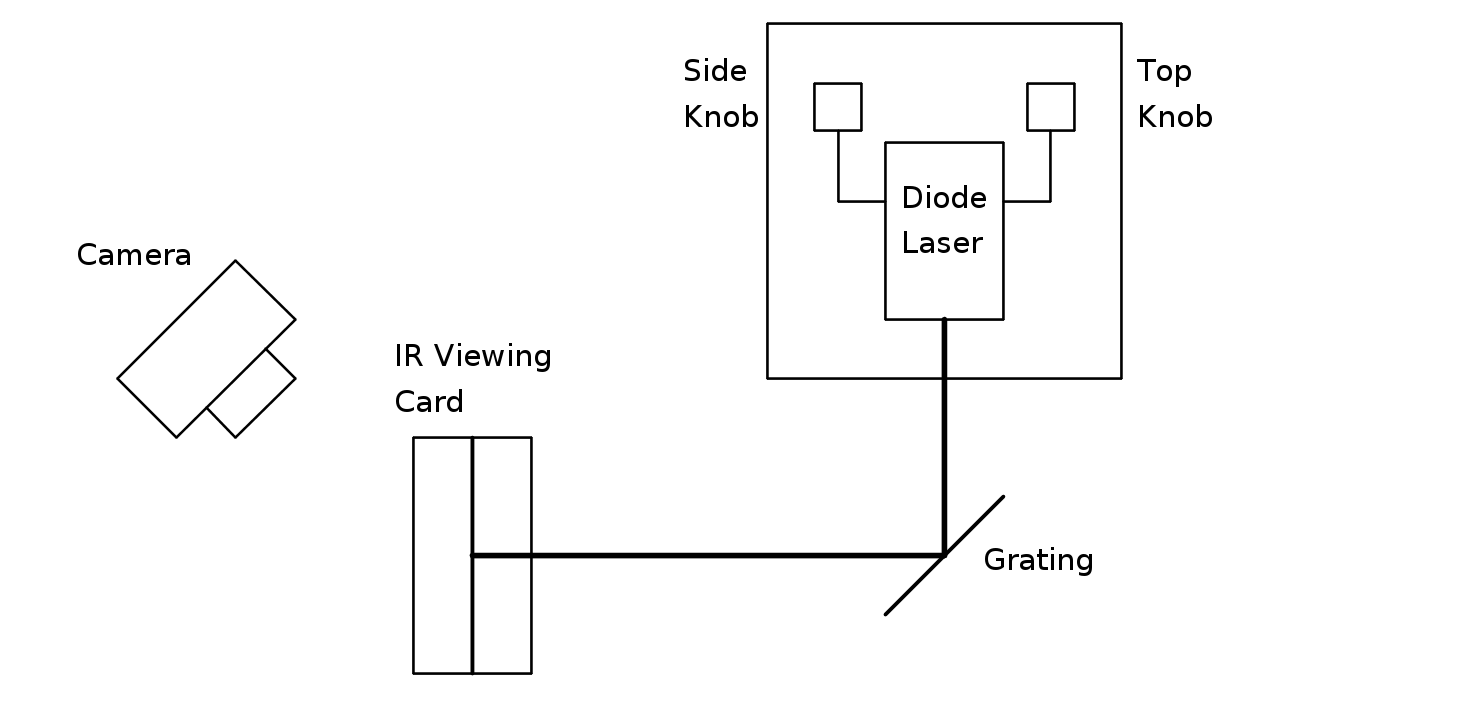
\includegraphics[width=\textwidth]{../pics/setup1.png}
 \caption{The laser beam, emitted by the diode gets detected by the IR card and can be seen with the camera.}
 \label{pic_setup1}
\end{figure}
With a camera the light spot can be seen on a TV monitor. Around the critical
voltage of 3.03-3.08 V a sharp slope in intensity of the light beam can be perceived which represents the transition of the beaming behaviour of the diode,
see also picture \ref{pic_stain}.
Below this critical voltage, the diode functions like an LED and above, stimulated emission dominates so that it serves as a laser. By slightly adjusting
the Top Knob and therefore the vertical orientation of the grating, the beam intensity gets maximized. the operating voltage is now a bit above the critical.
\begin{figure}
 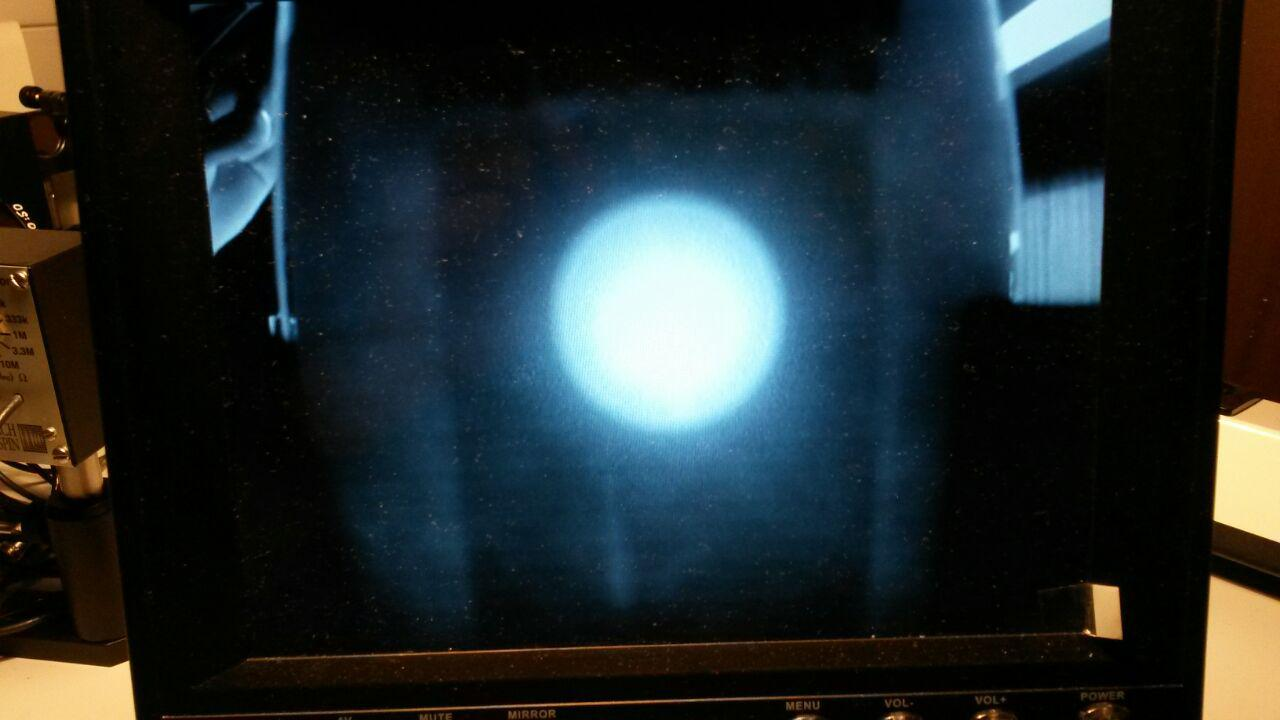
\includegraphics[]{../pics/bigstain.jpg}
\end{figure}


\subsection{Placement of the Rumdidium cell}
Now we place the RbC in a way that the laser passes through. The camera gets placed so that it looks into the cell and a photo diode (PD) measures the 
amplitude of the beam as depicted in figure \ref{pic_setup2}.
\begin{figure}[t]
 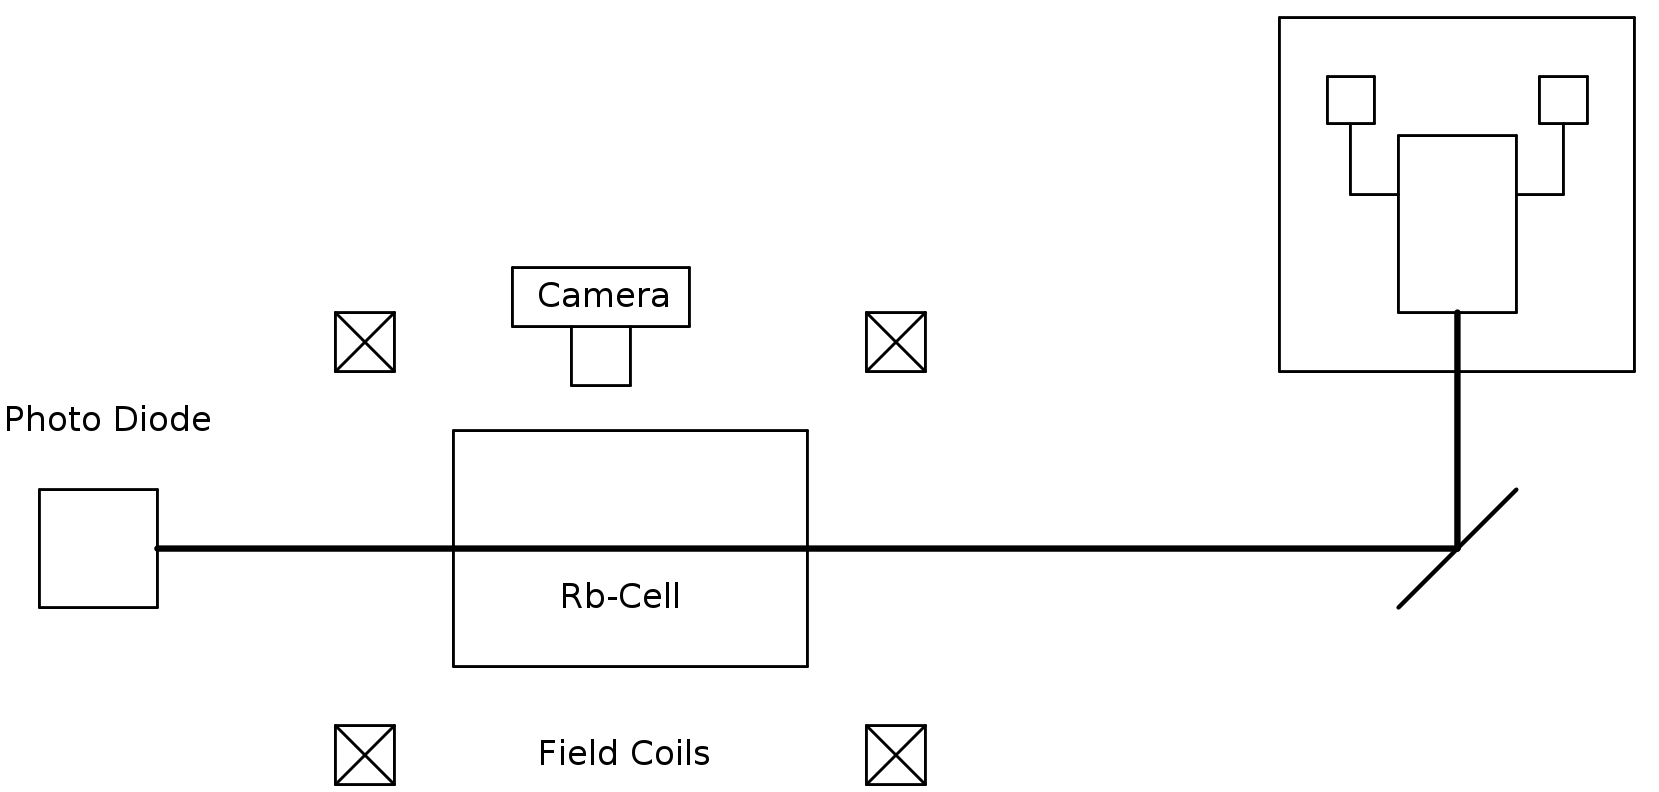
\includegraphics[width=\textwidth]{../pics/setup2.png}
 \caption{The beam passes through the RbC. Fluorescence effects can be seen on the monitor. The PD detects the beam amplitude}
 \label{pic_setup2}
\end{figure}
The ramp generator (RC) implemented in the LC gets linked to the also implemented piezo modulator (PM). The output voltage of RC is depicted by an 
oszillograph as the upper curve in figure \ref{pic_peak1}. With a frequency of 10 Hz at the RC, the grating gets modulated by the PM and therefore the 
frequency of the laser beam.
Now appearances of fluorescence in the RbC can be seen as blinkings on the screen. This can be further achieved by modifying the Side Knob.

\subsection{The Spectrum of Rubidium}
We saw fluorescence in the RbC and now we can display the spectrum of Rubidium. To achieve this, a glass neutral density filter gets placed before the RbC and
a photo diode (PD) right behind it. The PD gets connected to the oscillograph which displays its voltage.
\begin{figure}[t]
 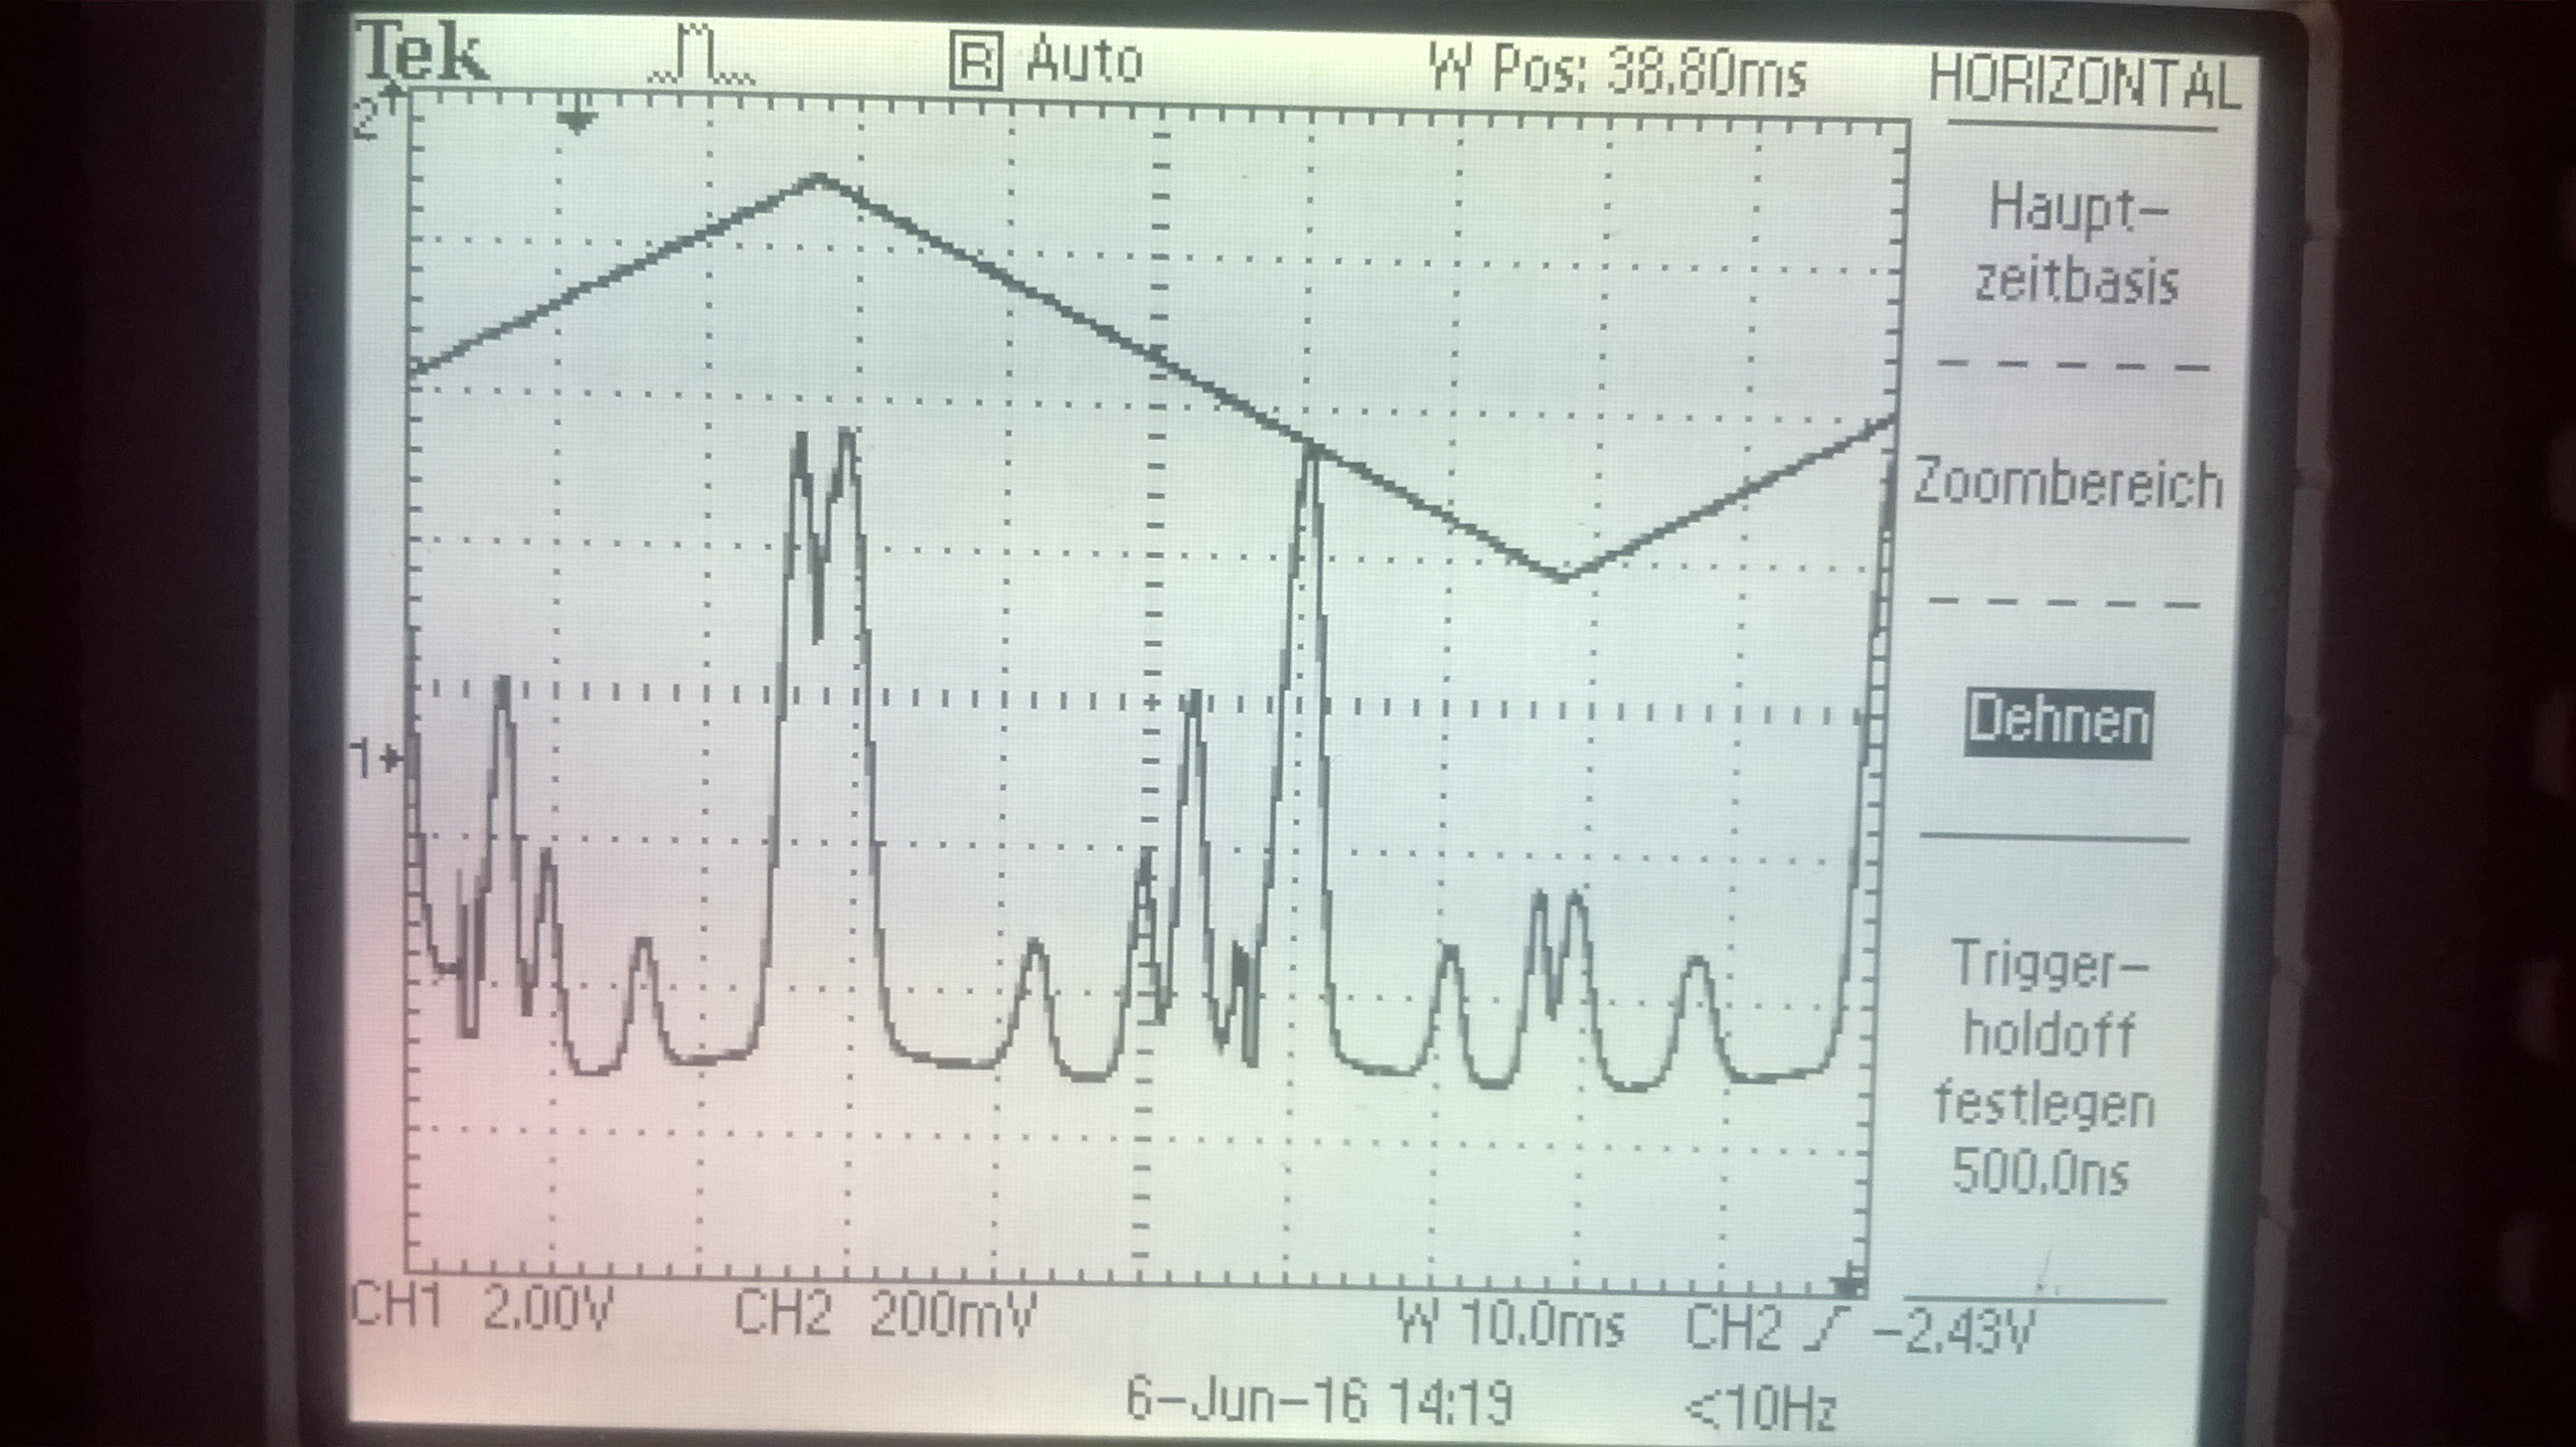
\includegraphics[width=\textwidth]{../pics/peaks.jpg}
 \caption{The output signal of the PM (upper) and of the PD (lower). Absorbtions and mode hoppings can be seen.}
 \label{pic_peak1}
\end{figure}
In figure \ref{pic_peak1} one can see that the beam is attenuated for certain frequencies. They can be identified in the following way. Light with a wavelength
$\lambda$ encounters the RbC. If it matches the exact difference between two energy levels the light gets absorbed by puting an electron from one level to
the other. By falling down to its former level a photon gets emitted isotropically and therefore the intensity of the original beam decreases.
With this method only the external resonater is modified by the PM and not the internal so that these jumps occur. So the laser does not pass through the 
frequencies continuously but skips at several ones.

\subsection{Simultaneous Modification of Current and PM}
To eliminate the jumps in the spectrum not only the PM but also the laser current will be modified. To do so, the modulation input gets connected with the 
RG. PM and current get modified simultaneously by the voltage produce by the RG. This means that now the external and internal resonator shift. Due to the 
increase (decrease) the beam intensity increases (decreases) the voltage of the PD shows a progression at which the absorbtion spectrum can be perceived
without jumps as in figure \ref{pic_peak1}.
\begin{figure}[H]
 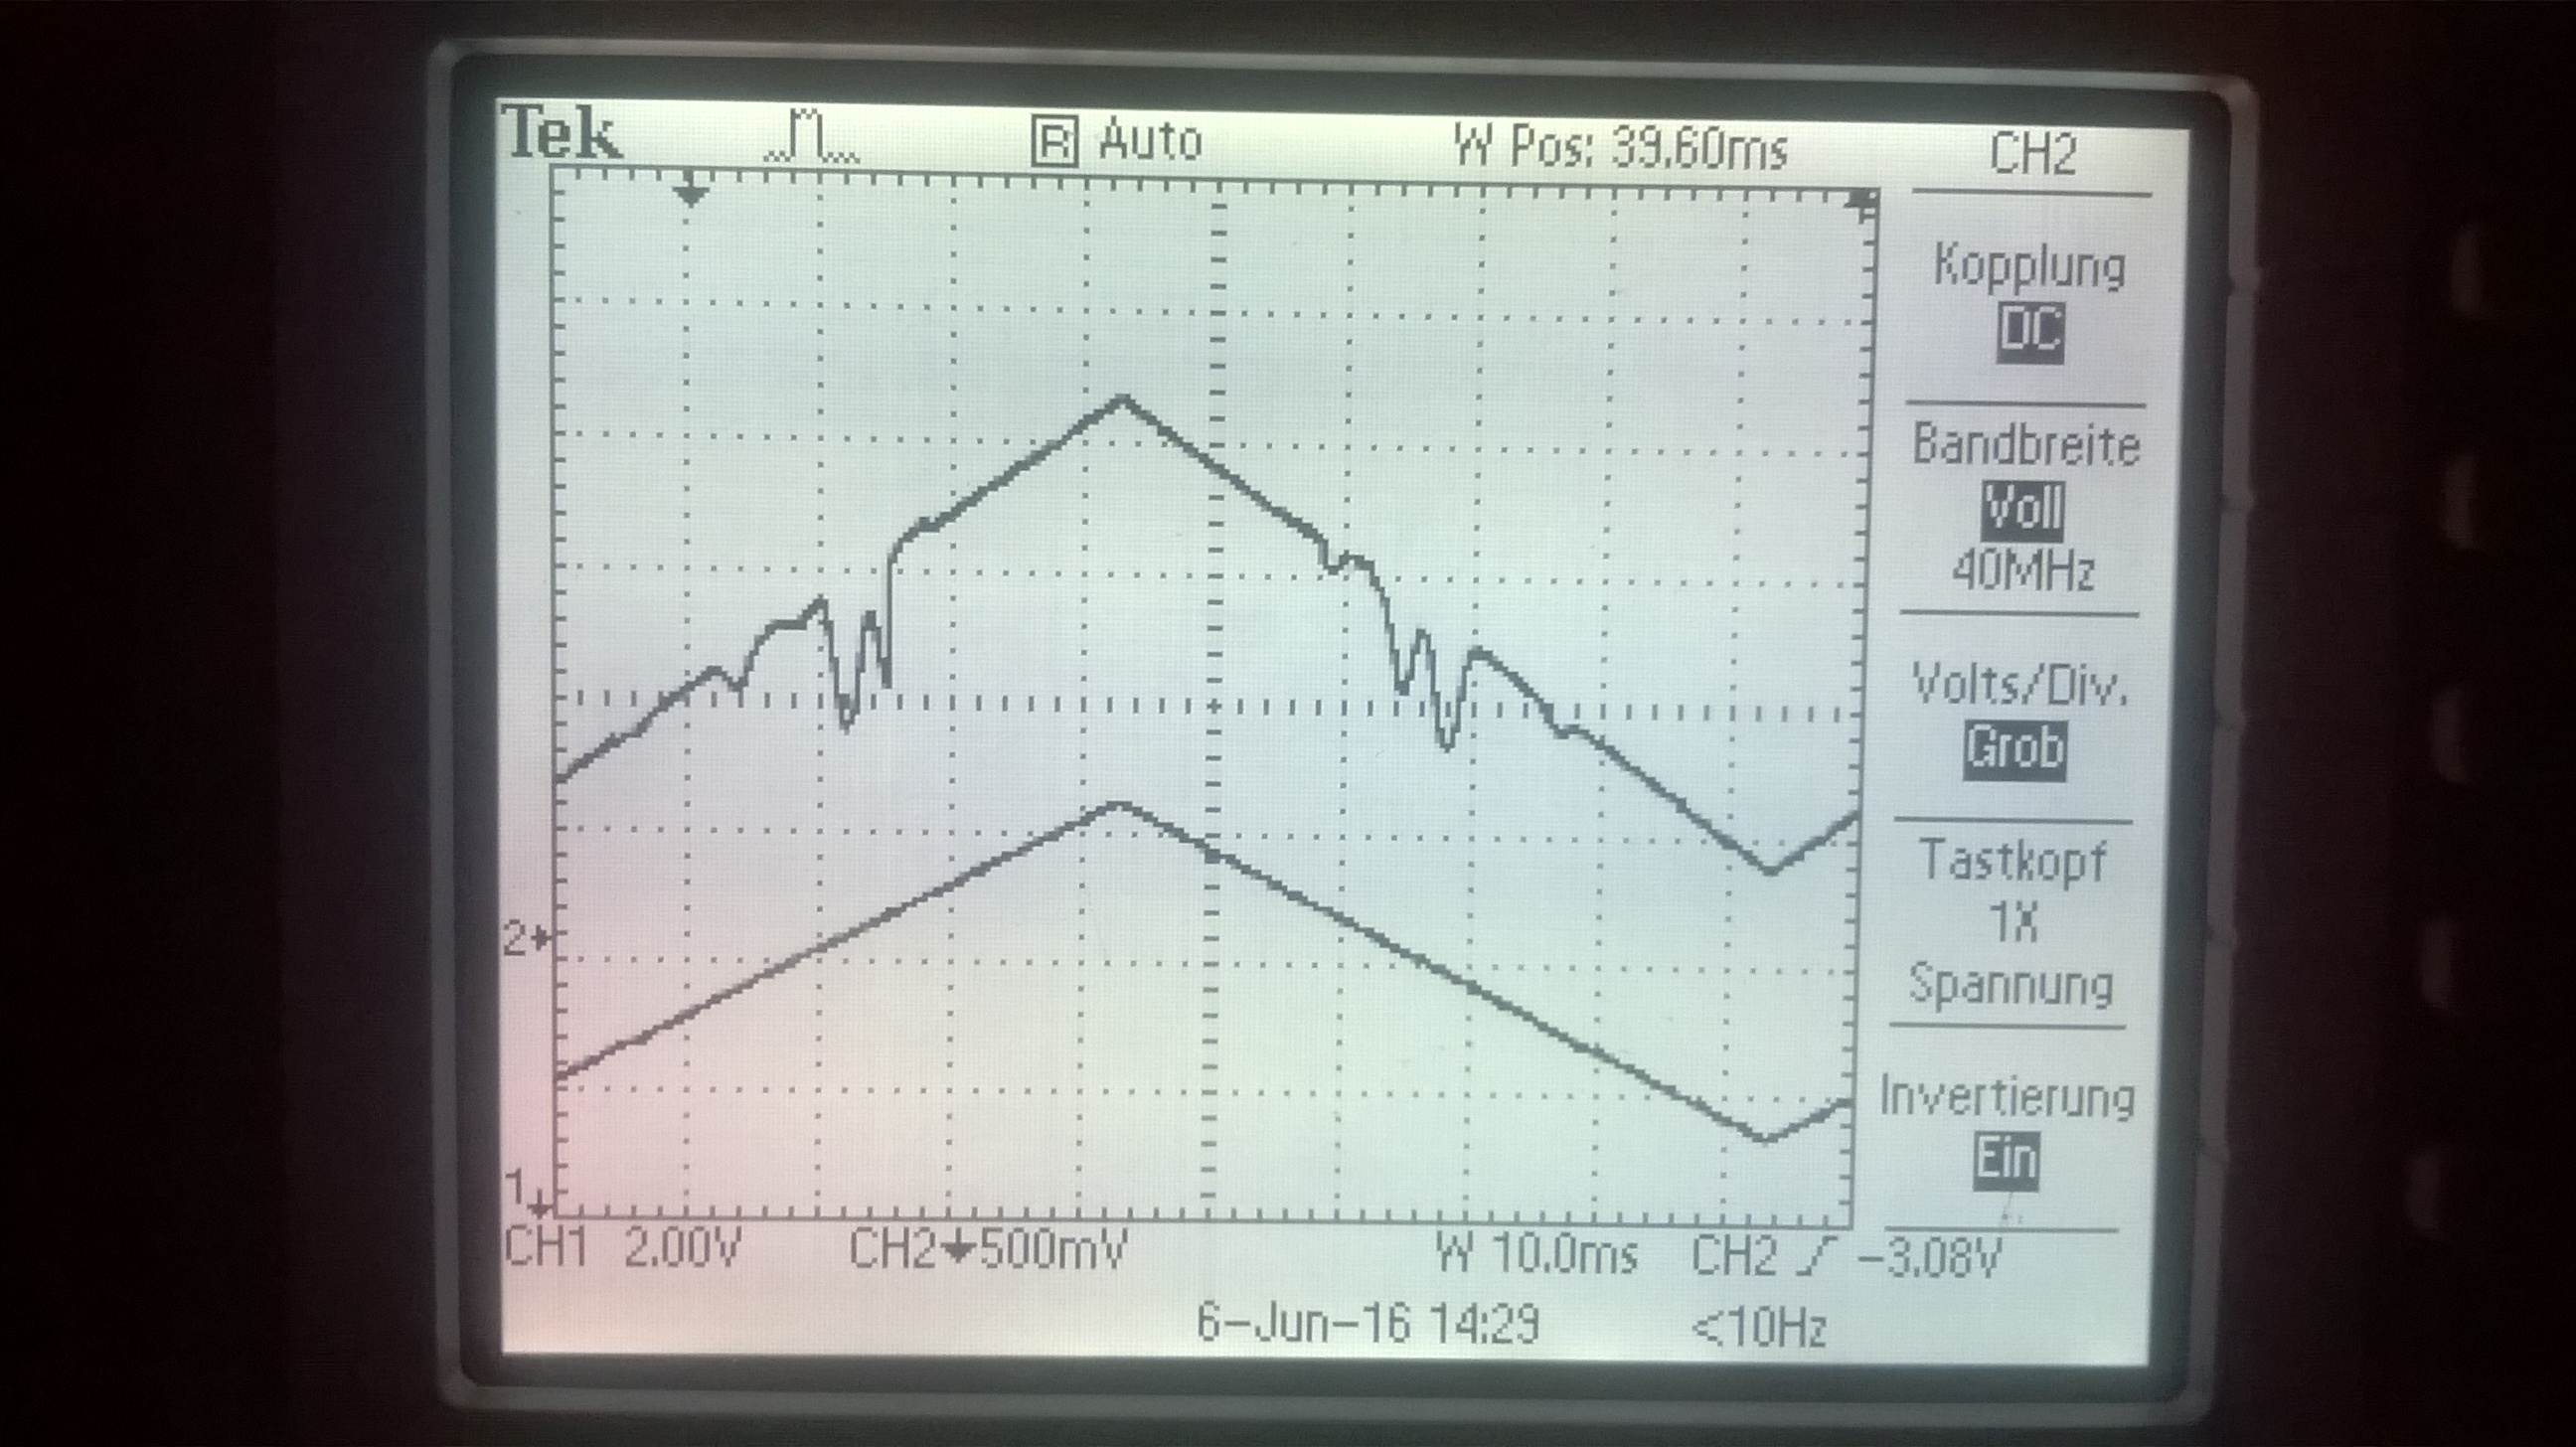
\includegraphics[width=\textwidth]{../pics/CandPM.jpg}
 \caption{The laser current gets modified by the RG as well as the PM. The absorbtion lines can now be seen without hoppings.}
 \label{pic_CandPM}
\end{figure}

\subsection{Representation of the Bare Absorbtion Spectrum}
Finally we want to represent the absorbtion spectrum of Rubidium without the ramp offset. By use of a semipermeable mirror (50:50) which splits the laser beam
into two equivalently intense beams before it crosses the RbC as in figure \ref{pic_setup3}. This beam is detected by a second photo diode PDII which only
plots the ramp offset without the Rubidium spectrum, though. Now the LC serves a function to balance two incoming signals. The input of PDI and PDII gets
balanced by a regulator so that the common offset cancels out and only the bare absorbtion spectrum remains. This spectrum can be seen in figure 
\ref{pic_spectrum}
\begin{figure}[H]
 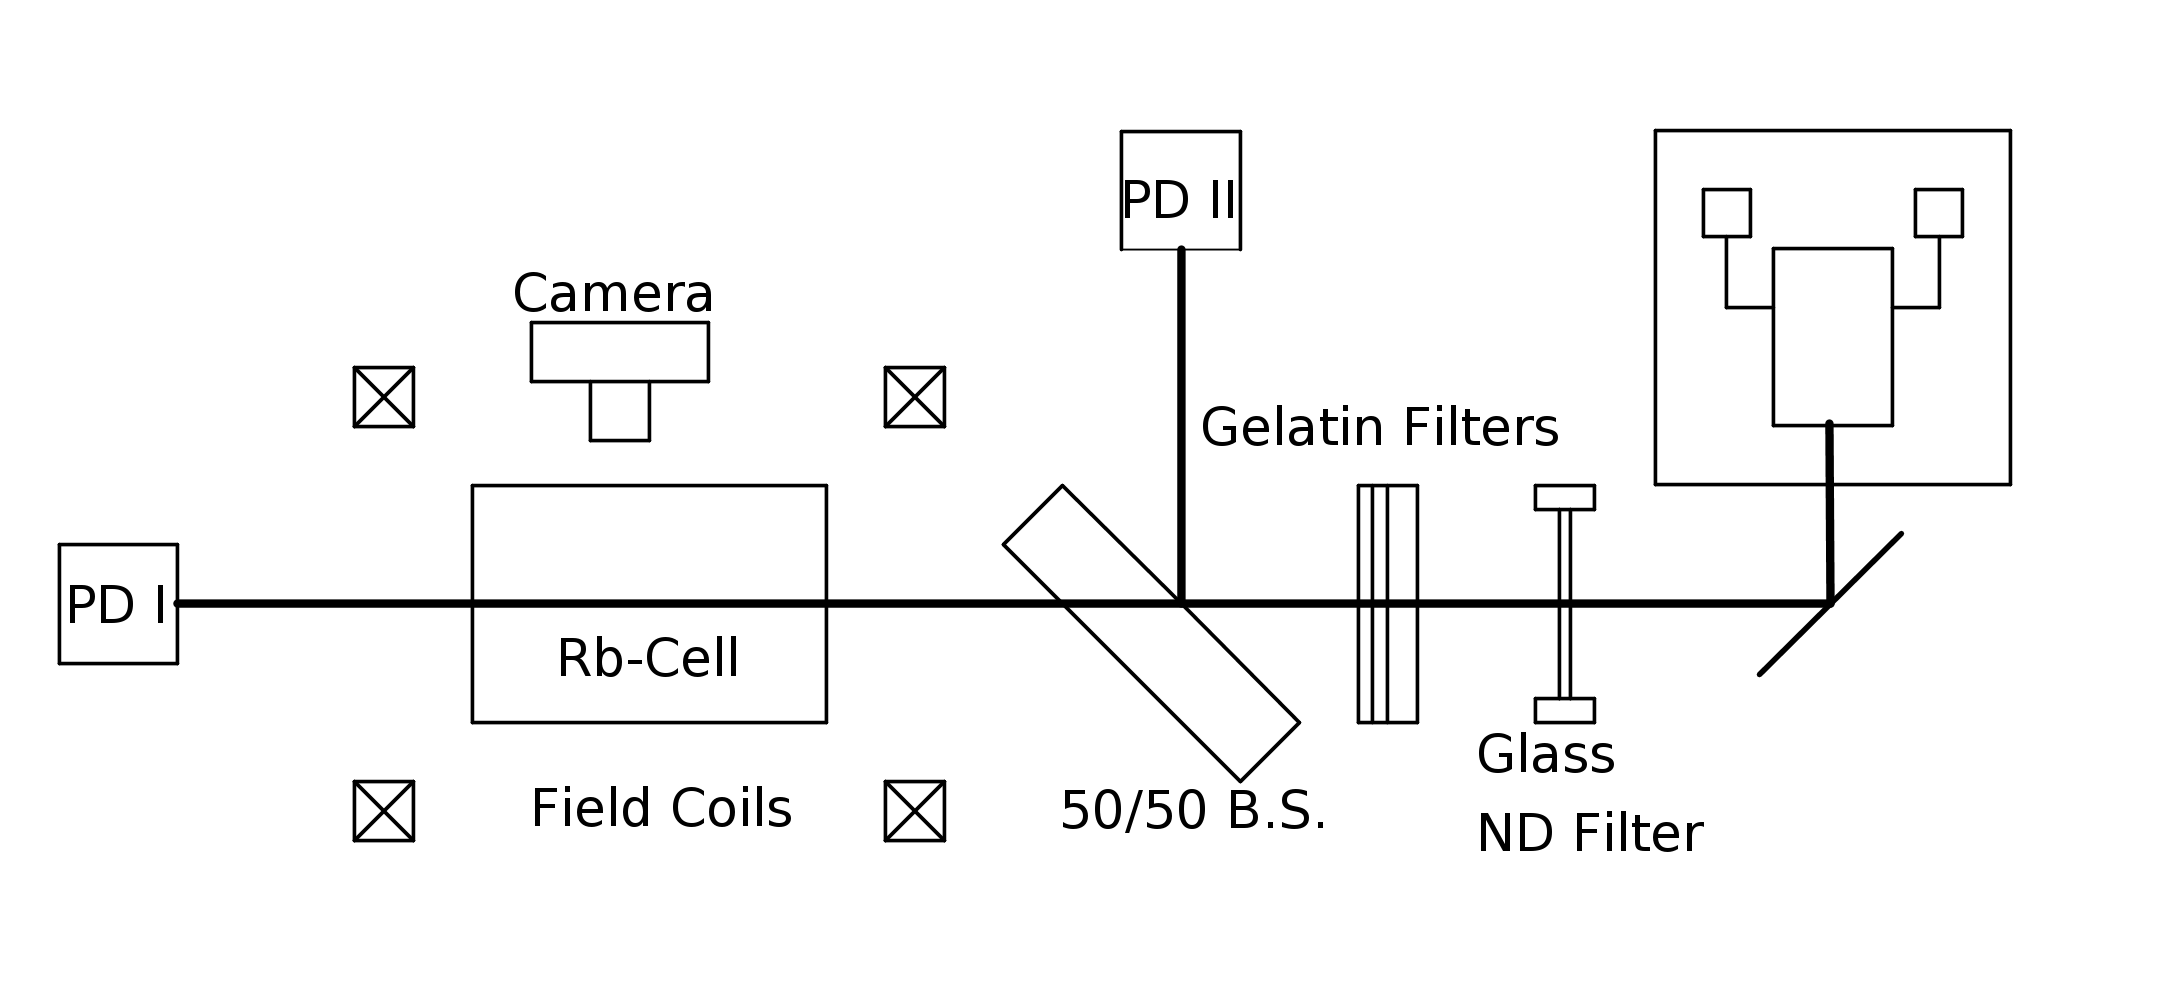
\includegraphics[width=\textwidth]{../pics/setup3.png}
 \caption{The 50/50 B.S. splits the beam. The signals of PDI and PDII differ by the ramp offset.}
 \label{pic_setup3}
\end{figure}

\begin{figure}[H]
 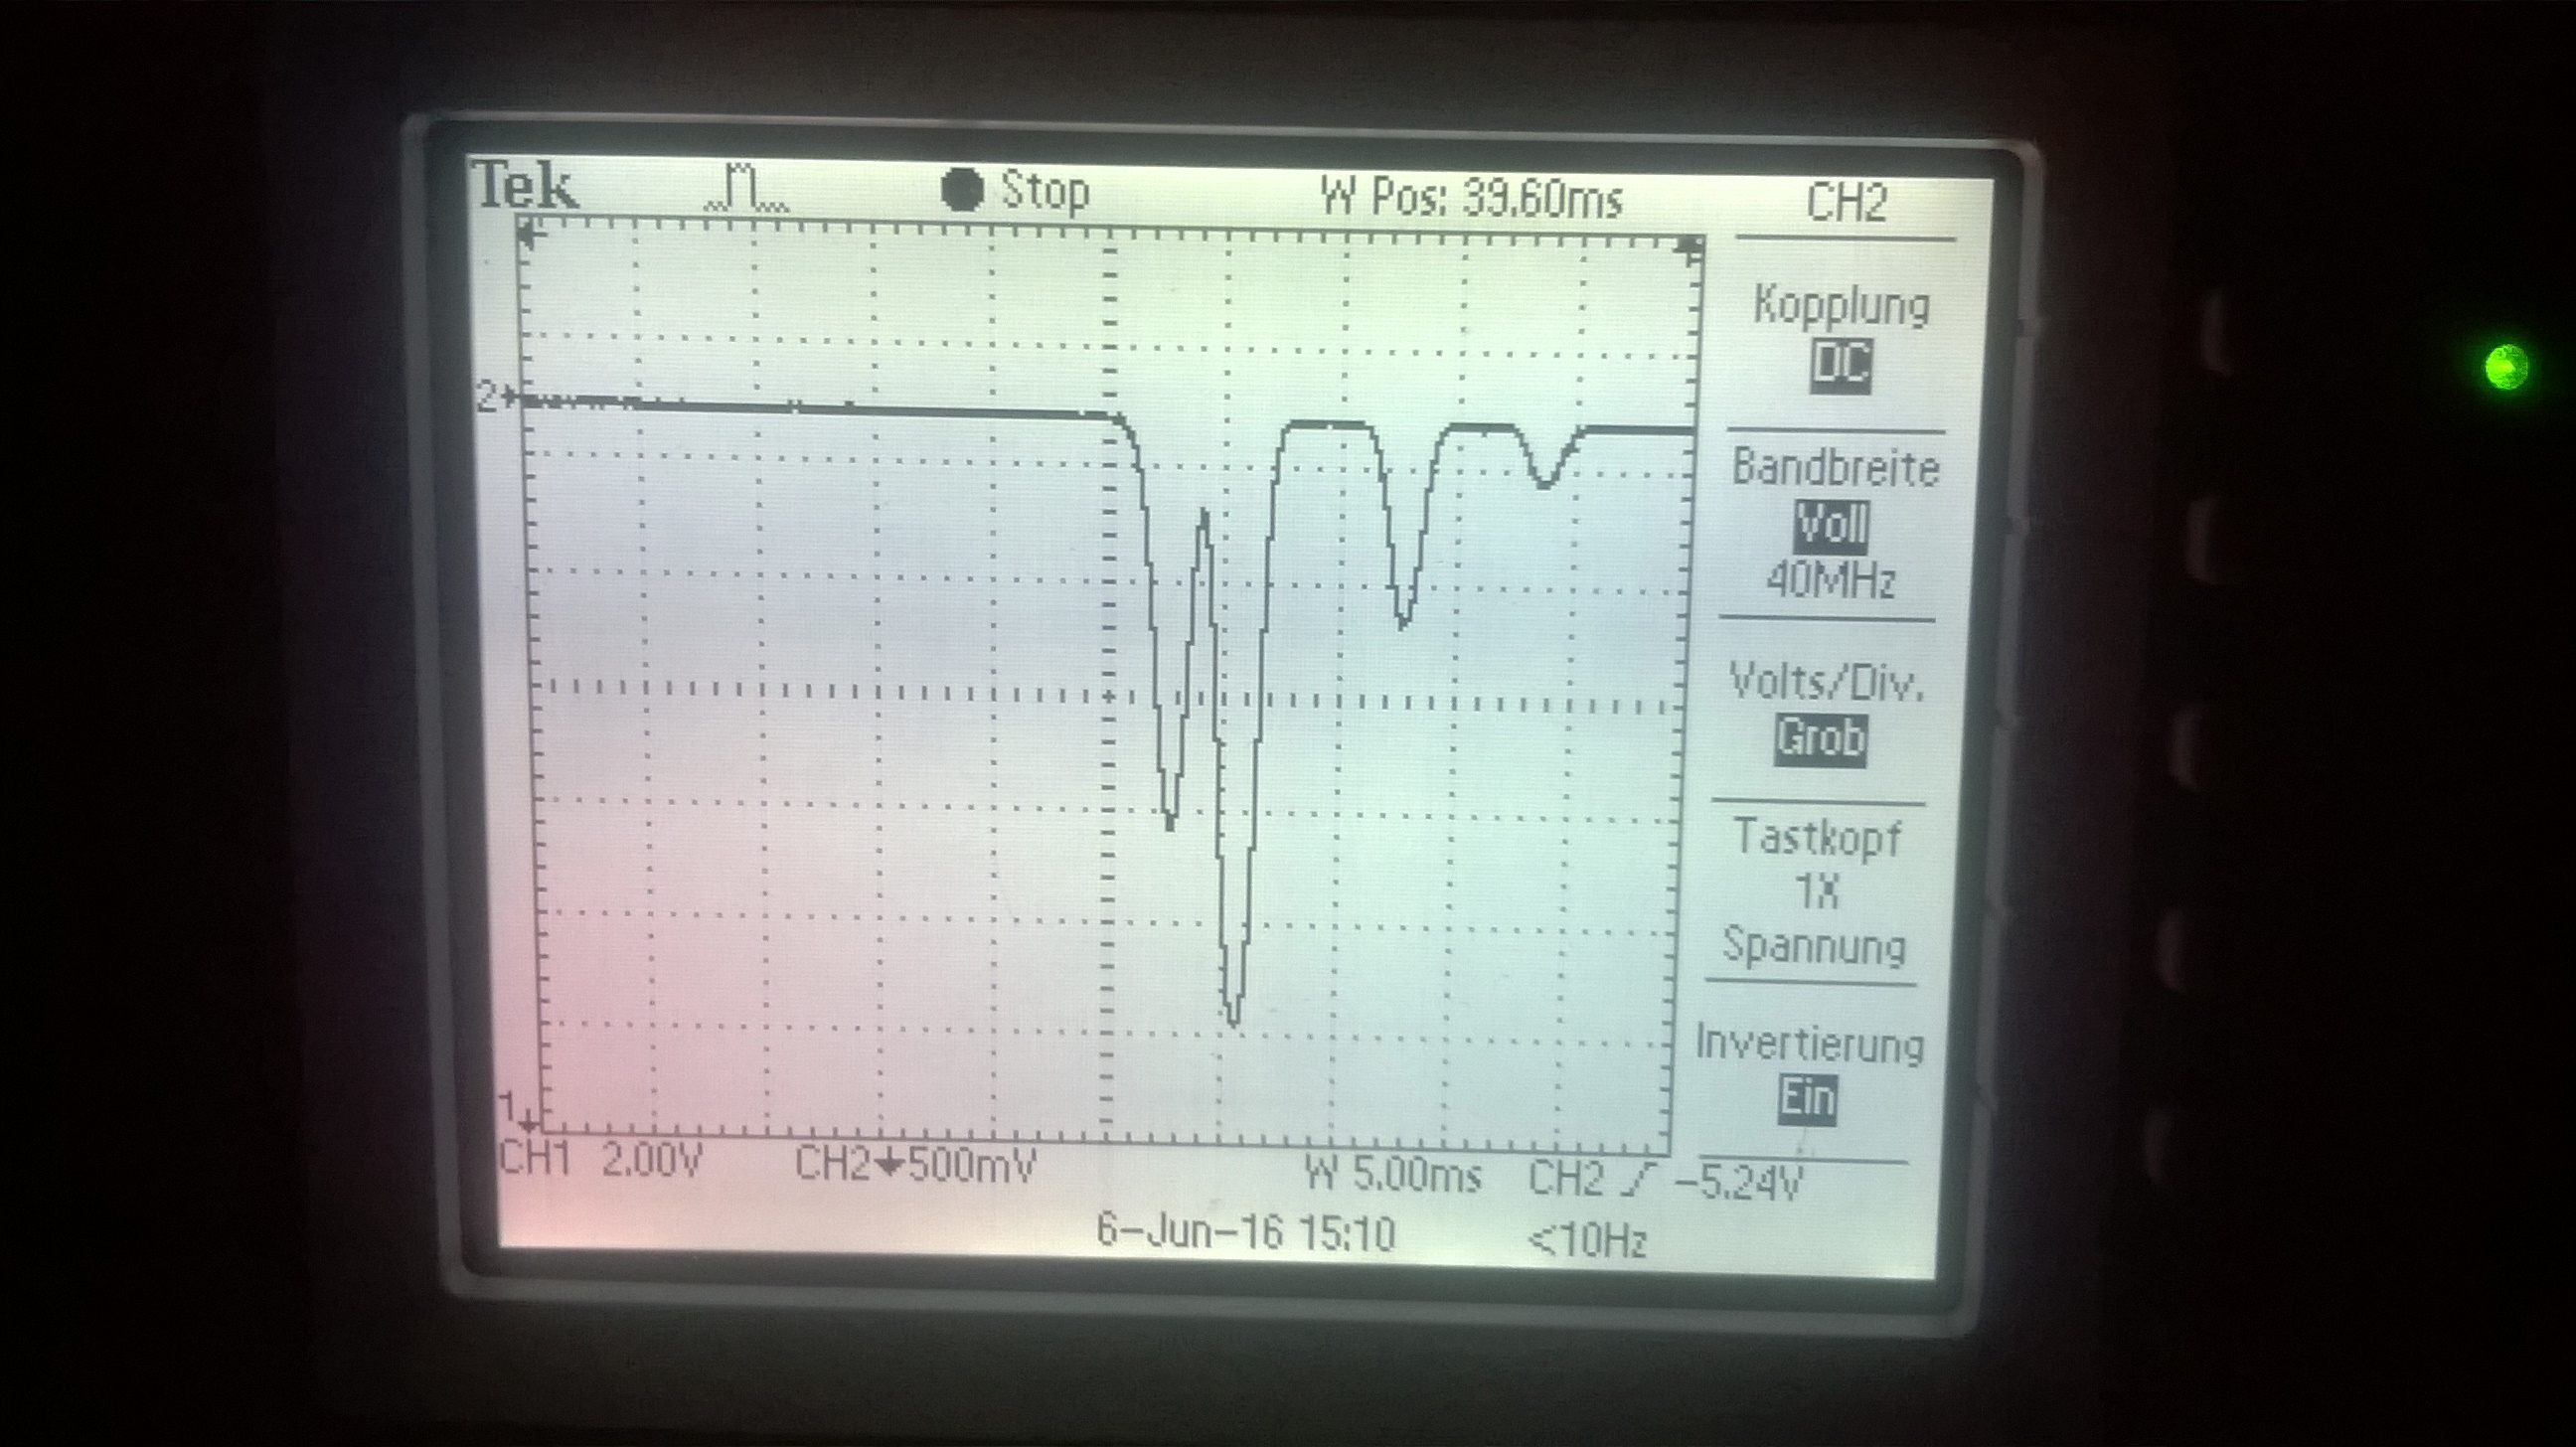
\includegraphics[width=\textwidth]{../pics/spectrum.jpg}
 \caption{The balanced signal is shown. The absorbtion spectrum of Rubidium can be seen clearly.}
 \label{pic_spectrum}
\end{figure}

\section{Discussion}
It can be said that with the very detailed manual it is quite easy to adjust a diode laser in a way that the absorbtion spectrum of such a sample as 
Rubidium can be probed and measured. A comparison of figure \ref{pic_spectrum} with a reference figure \ref{pic_ref} proves this ability and confirms that
the sample is indeed Rubidium.
\begin{figure}[H]
 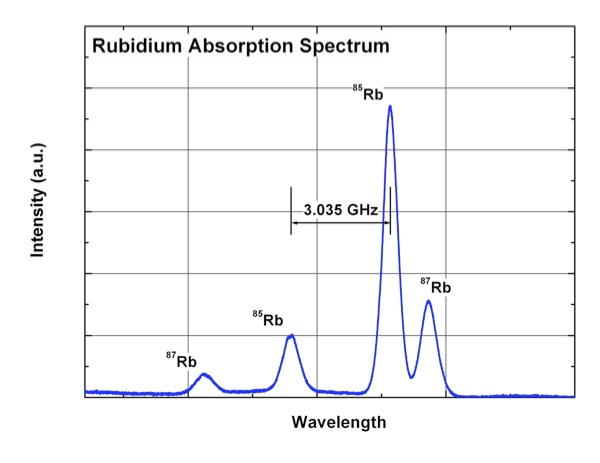
\includegraphics[width=0.7\textwidth]{../pics/reference.jpg}
 \caption{Absorbtion spectrum of Rubidium \cite{ref}}
 \label{pic_ref}
\end{figure}


\begin{thebibliography}{WissOnl}
	\bibitem{Anl} TU Dortmund instruction for experiment Nr.60 \url{http://129.217.224.2/HOMEPAGE/Anleitung_FPBSc.html}
	\bibitem{ref} Laser spectroscopy of rubidium \\ \url{http://www.photodigm.com/literature/applications-notes/rubidium-absorption-spectroscopy}
\end{thebibliography}

% ========================================
%	Literaturverzeichnis
% ========================================

%\bibliographystyle{plainnat}			% Bibliographie-Style auswählen
%\bibliography{BIBDATEI}			% Literaturverzeichnis

% ========================================
%	Das Dokument endent
% ========================================
\end{document}
